\documentclass[8pt]{article}
\usepackage[UTF8]{ctex}
\usepackage[a4paper]{geometry}

\usepackage{amsthm,amsmath,amssymb}
\usepackage{graphicx}
\usepackage{subfigure}
\usepackage{amsmath}
\usepackage{tabularx}
\usepackage{color}
\usepackage{hyperref}
\usepackage{ulem}
\usepackage{multirow}
\usepackage[cache=false]{minted}
\hypersetup{
	colorlinks=true,
	linkcolor=blue
}

\usepackage{appendix}
\geometry{a4paper,centering,scale=0.8}
\geometry{left=2.0cm, right=2.0cm, top=2.5cm, bottom=2.5cm}
\usepackage[format=hang,font=small,textfont=it]{caption}
\usepackage[nottoc]{tocbibind}

\usepackage{algorithm}
\usepackage{algorithmicx}
\usepackage{algpseudocode}
\usepackage{amssymb}
\usepackage{extarrows}
\usepackage{qcircuit}
\usepackage{fancyhdr}
\usepackage{cleveref}


\usepackage{tikz}  
\usetikzlibrary{arrows.meta}%画箭头用的包

\makeatletter
\def\@maketitle{%
	\newpage
	\begin{center}%
		\let \footnote \thanks
		{\LARGE \@title \par}%
		\vskip 1.5em%
		{\large
			\lineskip .5em%
			\begin{tabular}[t]{c}%
				\@author
			\end{tabular}\par}%
		\vskip 1em%
		{\large \@date}%
	\end{center}%
	\par
	\vskip 1.5em}
\makeatother

\newtheoremstyle{compact}%
{3pt}{3pt}%
{}{}%
{\bfseries}{\textcolor{red}{.}}%  % Note that final punctuation is omitted.
{.5em}{\mbox{\textcolor{red}{\thmname{#1}\thmnumber{ #2}}\thmnote{ (\textcolor{blue}{#3})}}}
\theoremstyle{compact}
\newtheorem{innercustomgeneric}{\customgenericname}
\providecommand{\customgenericname}{}
\newcommand{\newcustomtheorem}[2]{%
	\newenvironment{#1}[1]
	{%
		\renewcommand\customgenericname{#2}%
		\renewcommand\theinnercustomgeneric{##1}%
		\innercustomgeneric
	}
	{\endinnercustomgeneric}
}

\DeclareMathOperator{\card}{card}

\newtheorem{theorem}{定理}
\newtheorem{lemma}{引理}
\newtheorem{definition}{定义}
\newtheorem{proposition}{命题}
\newtheorem{corollary}{推论}
\newtheorem{example}{例}
\newtheorem{claim}{声明}
\newtheorem{remark}{注}
\newtheorem{thesis}{论点}
\newtheorem{Proof}{证明}

\def\obj#1{\textbf{\uline{#1}}}
\def\num#1{\textnormal{\textbf{\mbox{\textcolor{blue}{(#1)}}}}}
\def\le{\leqslant}
\def\ge{\geqslant}
\def\im{\text{im }}
\def\P#1{\mathbb{P}\left({#1}\right)}
\def\e{\mathrm{e}}
\def\E#1{\mathbb{E}\left[{#1}\right]}
\def\Var#1{\text{Var}\left[{#1}\right]}


\title{\heiti\zihao{2} 概率统计(A)课程作业: 概率论的基本概念}
\author{\kaishu\zihao{-3} 周书予\\2000013060@stu.pku.edu.cn}

\CTEXoptions[today=old]
\date{\today}

\begin{document}
\pagestyle{fancy}
\lhead{概率统计(A)}
\chead{2022 Spring}
\rhead{概率论的基本概念}


\crefname{theorem}{定理}{定理}
\crefname{lemma}{引理}{引理}
\crefname{figure}{图}{图}
\crefname{table}{表}{表}	
\maketitle

\section{}
	\begin{enumerate}
		\item 令$A_i = \varnothing\ (\forall i \in \mathbb N^+)$, 由可列可加性得$\P{\varnothing} = \sum\limits_{i=1}^{\infty}\P{\varnothing}$, 故$\P{\varnothing} = 0$.
		\item 令$A_1 = A, A_2 = B, A_i = \varnothing\ (\forall i \ge 3)$, 由可列可加性得$\P{A \cup B} = \P{A} + \P{B} + \sum\limits_{i=3}^{\infty}\P{\varnothing} = \P{A} + \P{B}$.	
		\item 由上一问得到$\P{A \cup B} = \P{A} + \P{B - A}$以及$\P{B} = \P{A \cap B} + \P{B - A}$, 结合两式得到$\P{A \cup B} = \P{A} + \P{B} - \P{A \cap B}$.
	\end{enumerate}

\section{}
	\begin{enumerate}
		\item
			\begin{itemize}
				\item $S = \{\textrm{red}, \textrm{green}, \textrm{white}\}$.
				\item $\mathcal F = \{\varnothing, 
				                     \{\textrm{red}\},
				                     \{\textrm{green}\},
				                     \{\textrm{white}\},
									 \{\textrm{red}, \textrm{green}\},
									 \{\textrm{red}, \textrm{white}\},
									 \{\textrm{green}, \textrm{white}\},
									 \{\textrm{red}, \textrm{green}, \textrm{white}\}
									 \}.$
				\item $\P{A} = \frac{|A|}{3}\ (\forall A \in \mathcal F).$
				\item 抽到白球的概率$= \P{\{\textrm{white}\}} = \frac13.$
			\end{itemize}
		\item
		\begin{itemize}
			\item $S = \{\textrm{white}, \textrm{not white}\}$.
			\item $\mathcal F = \{\varnothing, 
								 \{\textrm{white}\},
								 \{\textrm{not white}\},
								 \{\textrm{white}, \textrm{not white}\}
								 \}.$
			\item $\P{\varnothing} = 0, \P{\{\textrm{white}\}} = \frac13, \P{\{\textrm{not white}\}} = \frac23, \P{\{\textrm{white}, \textrm{not white}\}} = 1.$
			\item 抽到白球的概率$= \P{\{\textrm{white}\}} = \frac13.$
		\end{itemize}
	\end{enumerate}

\section{}
	\begin{enumerate}
		\item $\frac{(N-1)^{k-1}}{N^k}.$
		\item $\frac 1N$.
	\end{enumerate}

\section{}
	\begin{enumerate}
		\item $S = [0, 1] \times [0, 1].\ (x, y) \in S$表示两人分别在$7$点以后$x, y$小时的时候到达.
		\begin{center}
		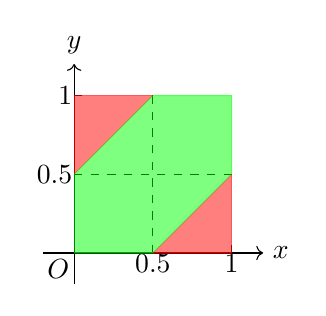
\begin{tikzpicture}[scale=2]
			\draw[->](-0.2, 0) -- (1.2, 0) node[right]{$x$};
			\draw[->](0, -0.2) -- (0, 1.2) node[above]{$y$};
			\draw[dashed](0.5, 0) -- (0.5, 1);
			\draw[dashed](0, 0.5) -- (1, 0.5);
			\node at (-0.1, -0.1) {$O$};
			\draw (0.5, 0) -- (0.5, 0.05) node[below]{0.5};
			\draw (1, 0) -- (1, 0.05) node[below]{1};
			\draw (0, 0.5) -- (0.05, 0.5) node[left]{0.5};
			\draw (0, 1) -- (0.05, 1) node[left]{1};
			\filldraw[green, opacity=0.5](0, 0) -- (0.5, 0) -- (1, 0.5) -- (1, 1) -- (0.5, 1) -- (0, 0.5);
			\filldraw[red, opacity=0.5](0.5, 0) -- (1, 0) -- (1, 0.5);
			\filldraw[red, opacity=0.5](0, 0.5) -- (0, 1) -- (0.5, 1);
		\end{tikzpicture}
		\end{center}
		
		$\P{\textrm{wait for at least half an hour}} = \P{\{(x, y) | |x - y| \ge 0.5\}} = \textrm{area of red triangles} = \frac14.$

		\item $S = [0, 1] \times [0, 1].\ (\alpha, \beta) \in S$表示选取的两个点分别是$\alpha A + (1 - \alpha)B, \beta A + (1 - \beta)B$(把$A, B$视作两个二维向量).
		
		\begin{center}
		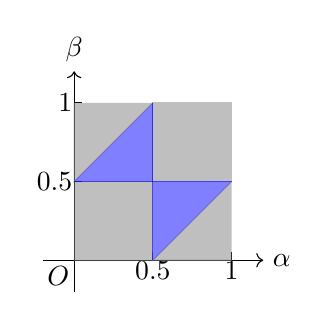
\begin{tikzpicture}[scale=2]
			\draw[->](-0.2, 0) -- (1.2, 0) node[right]{$\alpha$};
			\draw[->](0, -0.2) -- (0, 1.2) node[above]{$\beta$};
			\draw (0.5, 0) -- (0.5, 0.05) node[below]{0.5};
			\draw (1, 0) -- (1, 0.05) node[below]{1};
			\draw (0, 0.5) -- (0.05, 0.5) node[left]{0.5};
			\draw (0, 1) -- (0.05, 1) node[left]{1};
			\node at (-0.1, -0.1) {$O$};
			\filldraw[gray, opacity=0.5](0, 0) -- (0.5, 0) -- (0.5, 0.5) -- (0, 0.5);
			\filldraw[gray, opacity=0.5](1, 1) -- (0.5, 1) -- (0.5, 0.5) -- (1, 0.5);
			\filldraw[gray, opacity=0.5](0, 1) -- (0, 0.5) -- (0.5, 1);
			\filldraw[gray, opacity=0.5](1, 0) -- (0.5, 0) -- (1, 0.5);
			\filldraw[blue, opacity=0.5](0, 0.5) -- (0.5, 0.5) -- (0.5, 1);
			\filldraw[blue, opacity=0.5](0.5, 0) -- (0.5, 0.5) -- (1, 0.5);
		\end{tikzpicture}
		\end{center}

		$\P{\textrm{form a triangle}} = \textrm{area of blue triangles} = \frac14.$
	\end{enumerate}

\section{}

	由 i.i.d. 假设, 知$\P{A} = \P{B} = \P{C} = \frac13, \P{A \cap B} = \P{A \cap C} = \P{B \cap C} = \frac19$, 故$A, C$和$B, C$分别独立. 而$A \cap B \subseteq C$导致$\P{A \cap B \cap C} = \P{A \cap B} = \frac19 \neq \P{A}\P{B}\P{C}$, 所以$A, B, C$三者不互相独立.

\section{}

	定义事件$A = \{\mbox{至少一弹击中第一部分}\}, B = \{\mbox{两弹均击中第二部分}\}$, 由于$\P{A} = 1 - \P{\overline{A}} = 1 - 0.9^2 = 0.19, \P{B} = 0.2^2 = 0.04$, 且$A \cap B = \varnothing$, 故$\P{\textrm{plane shot down}} = \P{A \cup B} = \P{A} + \P{B} = 0.23.	$

\section{}

	\begin{enumerate}
		\item 令$S_n = \{\mbox{游戏在}\ n\ \mbox{轮后仍未终止}\}$, 归纳可知$\P{S_n} = \left( 1 - \frac{5}{36}\right)\left(1 - \frac 19\right)\P{S_{n-1}} = \left(\frac{62}{81}\right)^n$, $\lim\limits_{n \to \infty}\P{S_n} = 0$, 故有$1$的概率游戏会在有限步内终止.
		\item $\P{\mbox{甲获胜}} = \sum\limits_{n=0}^{\infty}\frac{5}{36}\P{S_n} = \frac{45}{76}.$
	\end{enumerate}

\section{}
	\begin{align*}
		\P{\mbox{恰有一个信封装有原来的信}} &= \sum_{i=1}^{4} \P{\mbox{第}\ i\ \mbox{个信封装有原来的信, 且其它信封都没有装原来的信}} \\
		&= \sum_{i=1}^{4} \frac14 \cdot \frac13\\
		&= \frac13
	\end{align*}

\section{}
	
	显然$\P{B_1} = \frac{b}{b+r}$. 对于$k \ge 2$, 考虑取出的球是第几次放入的, 即, 令$C_t = \{\mbox{取出的球是第}\ t \ \mbox{次放入的}\}$, 特别的, $C_0 = \{\mbox{取出的球初始时就在坛子里}\}$, 我们有

	\begin{align*}
		\P{B_k} &= \sum_{t=0}^{k-1}\P{B_k|C_t}\P{C_t} \\&= \frac{b}{b+r}\cdot\frac{b+r}{b+r+(k-1)c} + \sum_{t=1}^{k-1}\P{B_t}\cdot\frac{c}{b+r+(k-1)c} \\&= \frac{b + c\sum_{t=1}^{k-1}\P{B_t}}{b+r+(k-1)c}		
	\end{align*}

	根据归纳可知$\forall k \in \mathbb N^+, \P{B_k} = \frac{b}{b+r}$. 因此$\P{B_4} = \P{B_1} = \frac{b}{b+r}.$
\section{}

	令$A_i = \{\mbox{从第}\ i\ \mbox{只袋子里取出黑球}\}$, 则显然有$\P{A_1} = \frac{b}{a+b}$. 对于$k \ge 2$, 考虑有

	$$\P{A_k} = \P{A_k | A_{k-1}} \P{A_{k-1}} + \P{A_k | \overline{A_{k-1}}} \P{\overline{A_{k-1}}} = \frac{b + \P{A_{k-1}}}{a+b+1}$$

	根据归纳可知$\forall k \in \mathbb N^+, \P{A_k} = \frac{b}{a+b}$. 从而$\P{A_N} = \frac{b}{a+b}$.
\end{document}
